
\chapter{Etude préalable}
\section{Présentation de l’entreprise }
\subsection{Historique }
La Faculté de Chimie de l'USTHB (Université des Sciences et de la Technologie Houari Boumediene) 
est une institution éducative de renom en Algérie.\\
 L'USTHB est située à Alger, la capitale de l'Algérie. \\
 Bien que je n'aie pas accès à des détails spécifiques sur les événements ou développements récents à la faculté, 
 étant donné que ma base de connaissances s'arrête en septembre 2021, 
 je peux vous donner un aperçu général de son histoire jusqu'à cette date.\\
La Faculté de Chimie de l'USTHB a une longue histoire, remontant à la création de l'université elle-même.\\
 L'USTHB a été fondée en 1974 dans le cadre des efforts de l'Algérie pour promouvoir l'éducation en sciences et technologie dans le pays. \\

Au fil des ans, la Faculté de Chimie a joué un rôle important dans la formation 
et la production de professionnels qualifiés dans le domaine de la chimie.
\\ Elle propose des programmes de premier cycle, de cycles supérieurs et de doctorat, 
permettant aux étudiants de se spécialiser dans différents domaines tels que la chimie organique, 
la chimie inorganique, la chimie physique, la chimie analytique et la biochimie.\\

La faculté est dotée de laboratoires modernes, d'installations de recherche et d'enseignants expérimentés qui sont des experts dans leurs domaines respectifs.\\
La faculté met l'accent non seulement sur les connaissances théoriques, 
mais aussi sur les applications pratiques de la chimie à travers des expériences pratiques et des projets de recherche.\\
Cette approche aide les étudiants à développer une solide base en chimie et les prépare à des carrières dans l'enseignement,
l'industrie, la recherche et d'autres domaines connexes.\\

L'USTHB, y compris la Faculté de Chimie, est activement engagée dans la recherche scientifique et la collaboration avec d'autres universités et institutions de recherche,
tant au niveau national qu'international.\\
Les chercheurs et professeurs de la faculté ont contribué aux avancées dans divers domaines de la chimie, 
publiant des articles dans des revues scientifiques réputées et participant à des conférences et séminaires.\\

Au fil des ans, la Faculté de Chimie de l'USTHB a formé de nombreux diplômés qui ont ensuite apporté d'importantes contributions dans le domaine de la chimie en Algérie et au-delà.\\
 Leurs compétences et leurs connaissances ont contribué à façonner le développement des industries chimiques, 
 des études environnementales, de la pharmacie et d'autres domaines connexes dans le pays.\\
\newpage
\subsection{Missions}
La mission de la Faculté de Chimie de l'USTHB est de fournir une éducation de haute qualité dans le domaine de la chimie et de contribuer à la recherche scientifique dans ce domaine.\\
Voici les principaux aspects de sa mission :
  \begin{enumerate}
    \item \textbf{\large Enseignement :} La faculté vise à offrir des programmes d'enseignement de premier cycle, de cycles supérieurs et de doctorat en chimie. Elle vise à fournir aux étudiants une base solide de connaissances théoriques et pratiques en chimie, ainsi que les compétences nécessaires pour poursuivre une carrière dans des domaines tels que l'industrie chimique, la recherche scientifique, l'enseignement et d'autres secteurs connexes.

    \item \textbf{\large Recherche scientifique :} La faculté encourage la recherche scientifique dans différents domaines de la chimie, tels que la chimie organique, la chimie inorganique, la chimie physique, la chimie analytique et la biochimie. Les professeurs, chercheurs et étudiants sont encouragés à mener des projets de recherche novateurs, à publier des articles scientifiques et à participer à des conférences et séminaires nationaux et internationaux.

    \item \textbf{\large Collaboration et partenariats :} La faculté cherche à établir des collaborations et des partenariats avec d'autres institutions universitaires, des organismes de recherche et des industries, tant au niveau national qu'international. Ces collaborations visent à favoriser les échanges scientifiques, la mobilité étudiante et la mise en place de projets de recherche conjoints, contribuant ainsi à l'enrichissement mutuel et au développement de la chimie.

    \item \textbf{\large Service à la société :} La faculté s'engage à servir la société en mettant ses connaissances et son expertise en chimie au service du développement de l'industrie, de l'environnement, de la santé et d'autres domaines d'application. Elle vise à former des professionnels compétents et à contribuer à la résolution des problèmes sociaux, économiques et environnementaux grâce à des solutions chimiques innovantes.
  
  \end{enumerate}
En résumé, la mission de la Faculté de Chimie de l'USTHB est de former des chimistes qualifiés,
de promouvoir la recherche scientifique, de favoriser la collaboration et les partenariats,
et de mettre ses connaissances au service de la société.
\subsection{L’organigramme Générale }

\begin{figure}[hbtp]
  \centering
  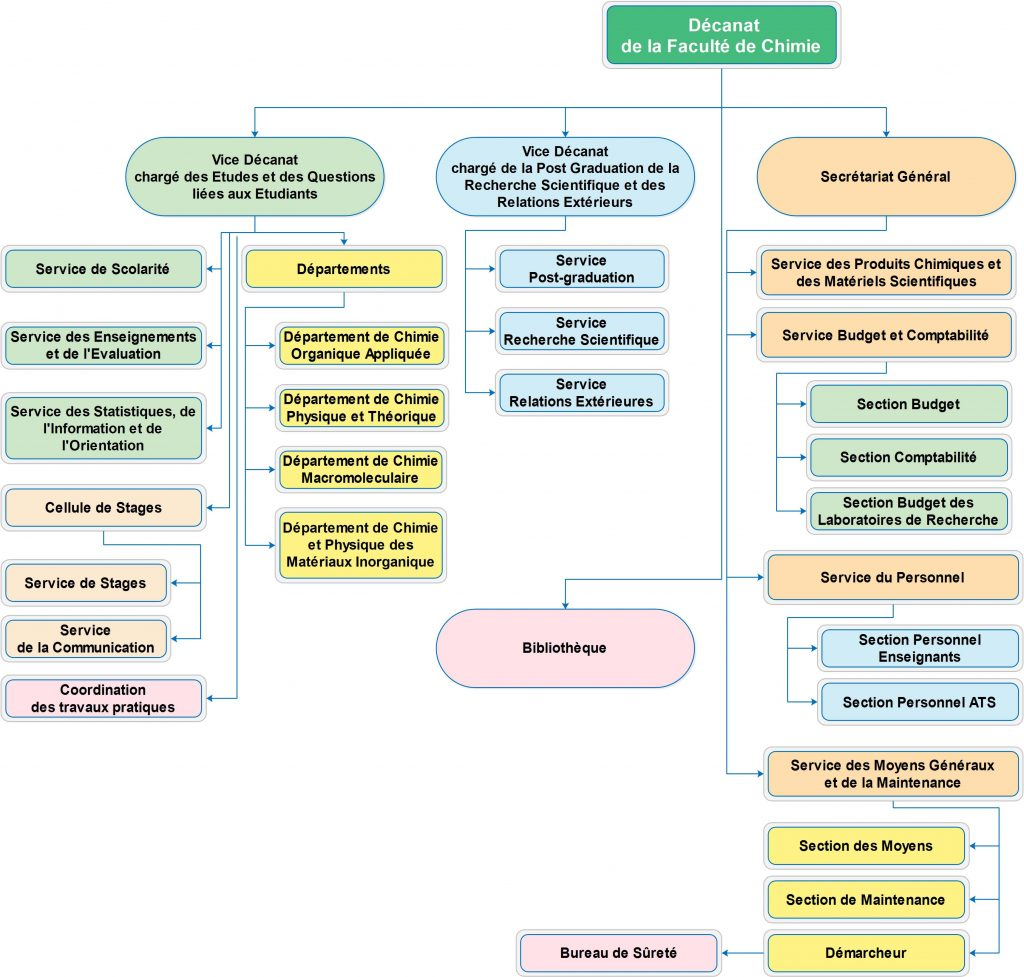
\includegraphics[width=.9\paperwidth]{images/org-gen.jpg}
  \caption{organigramme Générale}
  \label{fig:organigramme Générale}
\end{figure}
\newpage
\section{Présentation de sujet}
La présente étude s'inscrit dans le contexte des laboratoires d'analyse chimique au sein de la Faculté de Chimie.\\
 Ces laboratoires jouent un rôle crucial dans la formation des étudiants, 
 la recherche scientifique et la prestation de services analytiques à diverses industries et domaines de recherche.\\
 Cependant, ils sont confrontés à plusieurs défis qui impactent leur productivité et leur efficacité globale.
\subsection{Problématique du sujet}
Les laboratoires d'analyse chimique sont confrontés à des problématiques complexes liées à la gestion de leurs activités et de leurs ressources. \\
Parmi les principaux défis identifiés, on peut citer :
\begin{itemize}
  \item Le laboratoire de la faculté de chimie doit faire face à l'organisation et la planification efficace des rendez-vous pour les chercheurs, les étudiants et les intervenants extérieurs. De plus, il est crucial de gérer les disponibilités et l'état des équipements du laboratoire pour éviter les conflits d'utilisation
  \item La faculté de chimie doit suivre et documenter rigoureusement la provenance, la manipulation et les résultats des échantillons utilisés dans les expériences. Il est essentiel de garantir la traçabilité et la validité des données expérimentales
  \item Le laboratoire doit gérer efficacement son inventaire de produits chimiques et de verreries. Cela inclut le suivi des niveaux de stock 
  \item Le laboratoire doit rester à la pointe de l'innovation technologique pour maintenir sa compétitivité et sa pertinence dans le domaine de la chimie. Il est essentiel d'identifier et d'adopter les nouvelles technologies et les meilleures pratiques du secteur
\end{itemize}
\subsection{Objectifs du sujet}
L'objectif principal de cette étude est de concevoir et d'implémenter une application informatique sur mesure pour la gestion intégrée d'un laboratoire d'analyse chimique. Cette application vise à résoudre les problématiques identifiées et à atteindre les objectifs suivants :
\begin{itemize}
\item  Mettre en place un système de gestion des rendez-vous et des équipements intégré
\item  Mettre en place un système de traçabilité des échantillons et des expériences, avec des identifiants uniques, des fiches de suivi électroniques et des outils d'analyse de données
\item  Implémenter un système de gestion des stocks intégré, permettant le suivi en temps réel des produits et des verreries, la génération automatique de commandes
\end{itemize}
En résumé, la conception et la réalisation de cette application sur mesure pour la gestion de laboratoire d'analyse chimique représente un enjeu majeur pour l'amélioration de la qualité des services rendus par le laboratoire et pour l'optimisation de ses opérations. Cette initiative permettra de répondre aux défis actuels et futurs auxquels les laboratoires d'analyse chimique font face, tout en favorisant un environnement de travail efficace et innovant au sein de la Faculté de Chimie.
